
En cuanto terminamos la configuración inicial ya tenemos un servidor completamente funcional ofreciendo distintos servicios. Vamos a ver sus características por defecto y las formas que tenemos de modificarlos.

\section{Modos de administración}

Existen varios modos distintos de adminstrar el SME server.

\subsection{Consola de root de Linux}

Al arrancar el sistema, accedemos con el usuario "root" y la contraseña de administración. Esto nos proporciona un acceso al sistema operativo mediante la terminal de Linux.\\

\begin{figure}[H]
    \centering
    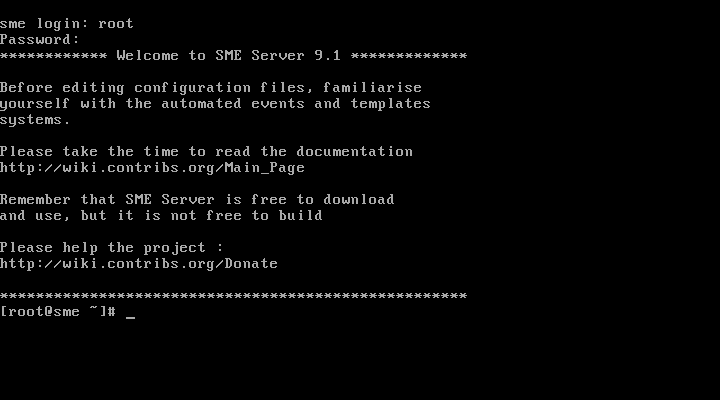
\includegraphics[width=\textwidth]{capitulo02/29.png}
\end{figure}

\subsection{Consola del servidor}

Al arrancar el sistema, accedemos con el usuario usuario "admin" y la contraseña de administración. También se puede acceder desde la consola de root, escribiendo "console".\\

\begin{figure}[H]
    \centering
    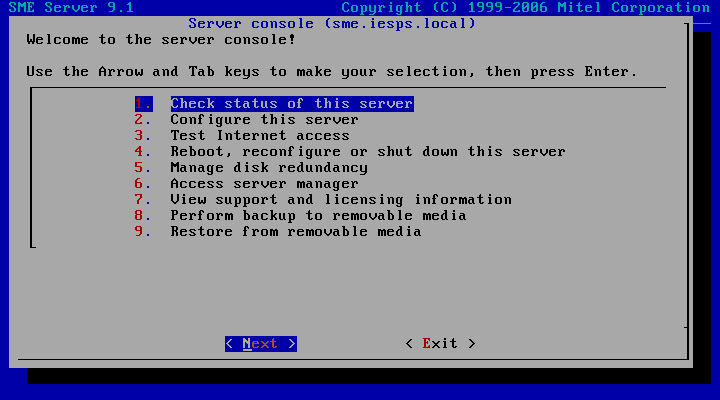
\includegraphics[width=\textwidth]{capitulo03/00.png}
\end{figure}

Tiene varias opciones
\begin{enumerate}
 \item \textbf{Check status of this server}: muestra el tiempo que ha estado en marcha el servidor.
\item \textbf{Configure this server}: nos lleva otra vez a través de las pantallas de la configuración inicial por si queremos cambiar algo.
\item \textbf{Test internet access}: prueba el acceso a internet mandando datos a contribs.org.
\item \textbf{Reboot, reconfigure or shut down this server}: reiniciar, reconfigurar o apagar el servidor.
\item \textbf{Manage disk redundancy}: muestra el estado de los discos y permite administrar el tipo de RAID. En nuestro caso solo hay un disco instalado... Parece que ha hecho 2 particiones (MIRAR).
\item \textbf{Access server manager}: permite acceder a la interfaz de administración web server-manager desde el mismo servidor usando el navegador en modo texto ELinks.
\item \textbf{View Support and licensing information}: ver la licencia (GNU GPL) e información sore cómo contactar con contribs.org para el soporte.
\item \textbf{Perform backup to removable media}: permite hacer un backup del estado actual del servidor en una unidad USB. La imagen se comprime en un archivo .tgz.
\item \textbf{Restore from removable media}: permite recuperar una imagen del servidor anteriormente guardada en una unidad USB.
\end{enumerate}

\subsection{Aceso remoto}
Podemos acceder a estos dos modos de administración desde otro PC a través de SSH, pero está desactivado por defecto:

\begin{figure}[H]
    \centering
    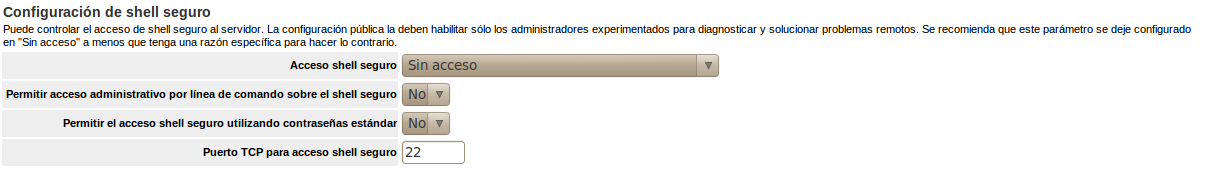
\includegraphics[width=\textwidth]{capitulo03/ssh00.png}
\end{figure}

En esta práctica permitiremos el acceso por SSH desde las redes locales para una administración más sencilla. Una vez activado, tendremos disponibles las dos primeras formas de administración que hemos explicado, dependiendo de si nos conectamos como 'root' o como 'admin'. SME server permite también el acceso mediante PPTP para la administración.

\subsection{Interfaz web server-manager}

SME Server provee una interfaz web de administración. Se accede desde el navegador de cualquier ordenador de la red interna con cualquiera de las siguientes URL:

\begin{itemize}
  \item https://sme/server-manager
  \item https://192.168.0.254/server-manager
\end{itemize}

\begin{figure}[H]
    \centering
    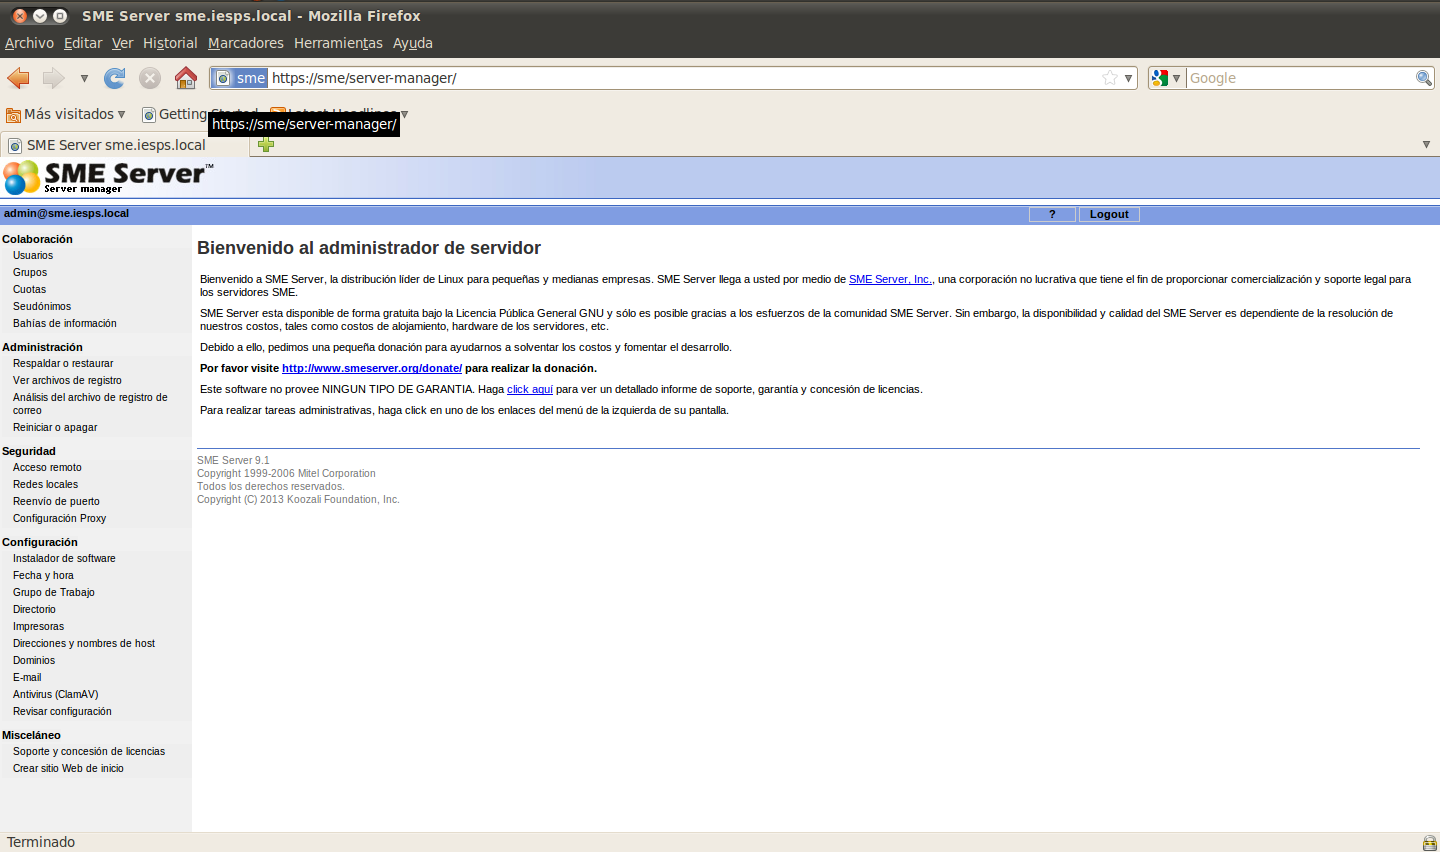
\includegraphics[width=\textwidth]{capitulo03/11.png}
\end{figure}
\newpage 
\section{Servicios y caracerísticas}

\subsection{Usuarios}

Las cuentas de usuario en SME server incluyen cuentas de email y áreas de almacenamiento separadas y protegidas por contraseña.

-> Opcion de reenvio para los emails

-> Como cambiar la password desde el navegador web

-> The user group function serves two purposes in the SME Server: it permits email to be sent conveniently to a group of users, and it allows the system administrator to associate groups of users with a single information bay (i-bay).

-> By default, there is no size limit on the files a user may store on the server nor the amount of email that can be received. However, if you wish to limit the disk space a particular user account can use, you may do so on the " Quotas " panel in the server-manager.

\subsection{email}

Configuración general

\begin{figure}[H]
    \centering
    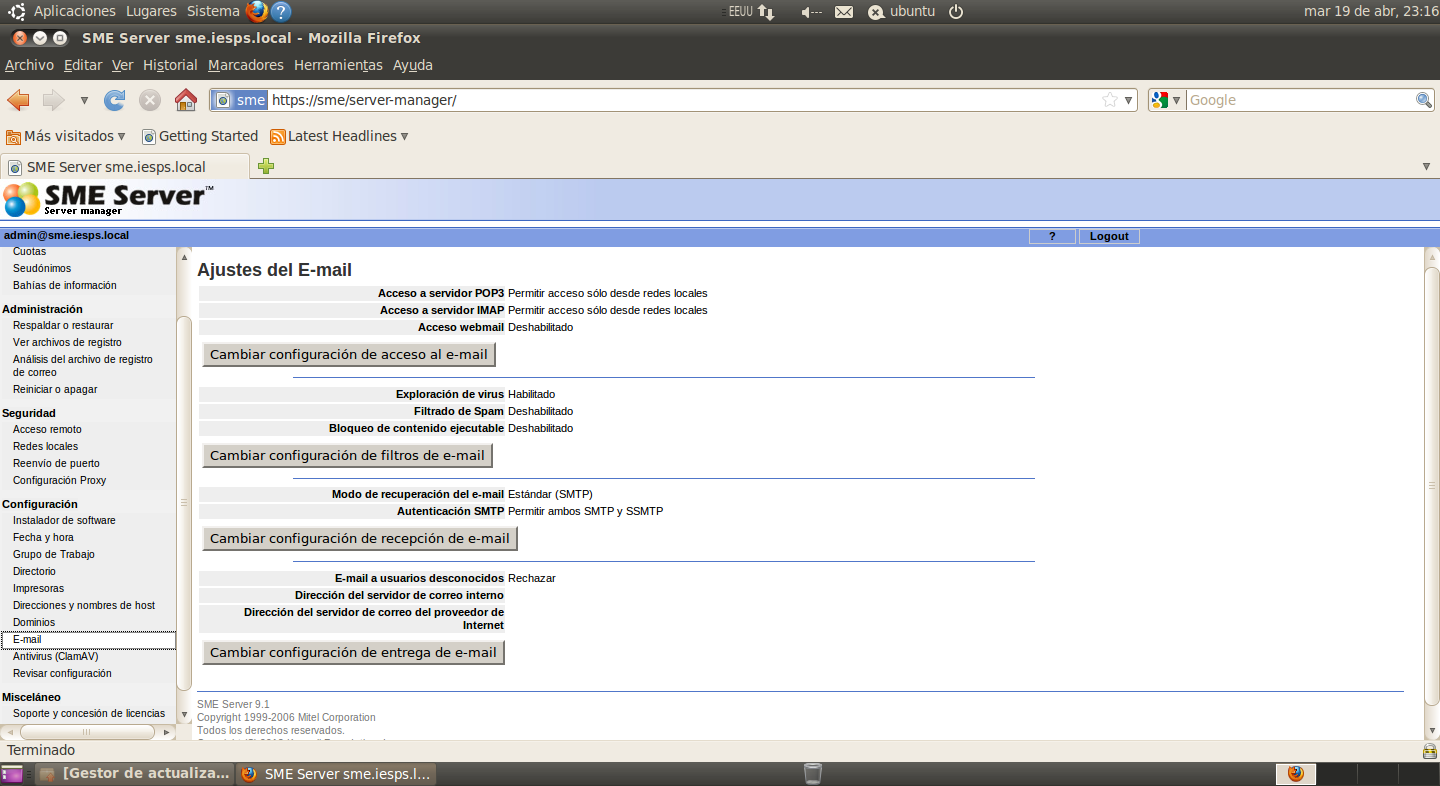
\includegraphics[width=\textwidth]{capitulo03/13email.png}
\end{figure}

\subsection{Almacenamiento, i-bays}

\subsection{DNS}

...


